\section{Root Locus based Design}\label{rLocus}
The Root Locus of a transfer function is a plot of all the possible positions of the closed loop poles when applying a proportional gain K. The number of poles will be the same as the ones in the open loop case and every of them will have an associated branch that shows how it will change with K. The plot has the following main characteristics:

\begin{itemize}
	\item[-] The plot is symmetric with respect to the real axis.
	\item[-] The number of branches is equal n, which is the number of poles in the open loop function.
	\item[-] There are m branches that ends in the zeros of the open loop function, being m the number of zeros.
	\item[-] There are n-m branches that go to infinity.
	\item[-] The position of the poles changes the behavior of the system as seen in \figref{rLocusStability}
\end{itemize}

\begin{figure}[H] 
	\centering 
	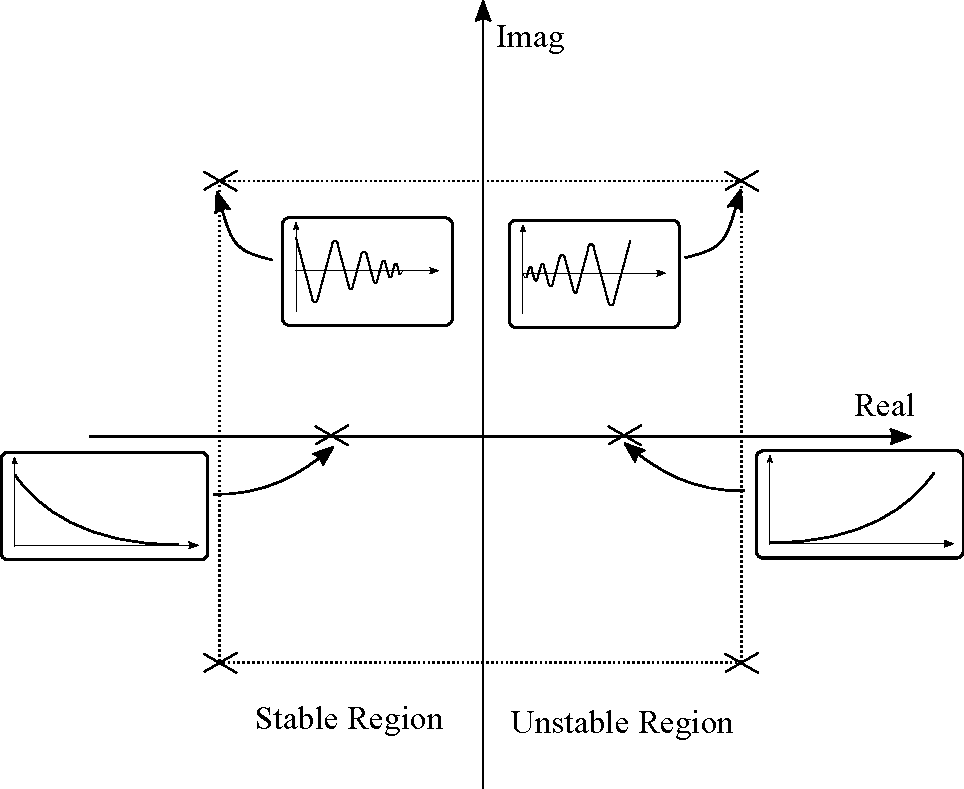
\includegraphics[scale=0.5]{figures/rLocusStability}	
	\caption{Nyquist plot of the system with the controller}
	\label{rLocusStability}
\end{figure}
%
Root Locus design of controllers is based on the fact that the closed loop poles of a system will depend on the poles, zeros ans gain of the open loop function. Knowing how the plot changes with the addition of poles and zeros, the branches can be modified to place the poles of the closed loop function where needed. When using this design method, the final system look like \figref{blockDiagramController}.

\begin{figure}[H]
	\begin{tikzpicture}[ auto,
thick,                         %<--setting line style
node distance=1.5cm,             %<--setting default node distance
scale=0.75,                     %<--|these two scale the whole thing
every node/.style={scale=0.62}, %<  |(always change both)
>=triangle 45 ]

%-- Blocks creation --%
\draw
% DIRECT TERM %
node[shape=coordinate][](input1) at (0,0){}
node[shape=coordinate][](feed) at (0.5,0){}
node(sum1) at (2,0) [sum] {$\sum$}
node(controller) at (4,0) [block]{\Large $D(s)$}
node(plant) at (6,0) [block]{\Large $G(s)$}
node[shape=coordinate][](DummyNode) at (5,-1.5){}
node[shape=coordinate][](FeedbackNode) at (7.5,0){}
;

%-- Block linking --%
% INPUT %
\draw[-](input1)        -- node{\Large $U(s)$}(feed);
\draw[->](feed)  -- (sum1);

% OUTPUT %
\draw[-](plant)  -- (FeedbackNode);
\draw[->](FeedbackNode)       -- node {\Large $Y(s)$} (9,0);

% DIRECT TERM %
\draw[->] (sum1)            -- (controller);
\draw[->] (controller)       -- (plant);

% FEEDBACKS %
\draw[-] (FeedbackNode)  |- (DummyNode);
\draw[->] (DummyNode)  -| (sum1);

%-- Nodes --%
\draw%--------------------------------------------------------------
node at (input1)            [shift={(-0.04, -0.05 )}] {\Large \textopenbullet}
node at (FeedbackNode)      [shift={(0, -0.07 )}] {\Large \textbullet}
;
%-- Summation signs --%
\draw%--------------------------------------------------------------
node at (sum1) [right = -6.6mm, below = .6mm] {$+$}
node at (sum1) [right = -3mm, below = 3.9mm]  {$-$}
;

\end{tikzpicture} 
	\centering
	\caption{Block diagram of the system}
	\label{blockDiagramController}
\end{figure}

